\chapter{Der Weg zu DevOps} % Feel free to rename

Bis hierhin haben wir alles wichtige über DevOps gelernt. Seine Vor- und Nachteile, was es lösen kann und auch was es nicht lösen kann. Aber vorallem ist klar, dass DevOps nicht kaufbar ist. Zumindest nicht wie man eine Software kauft, installiert und dann vergessen kann. Darum gestaltet sich die Einführung von \ac{DevOps} in eine bereits bestehende Unternehmenskultur als schwierig.

Ein Ansatz um dieses Problem an zu gehen wird im nächsten Unterkapitel beschrieben, sowie nachfolgend ein Blick auf die Anwendung von \ac{DevOps} in der realen Welt.


\section{Der Three-Way-Approach}

Der Three-Way-Approach versucht sich an der Etablierung von \ac{DevOps} über 3 Stufen. \cite{nine:2018}

\begin{enumerate}
\item Das Flow Prinzip
\item Das Feedback Prinzip
\item Das Prinzip des kontinuierlichen Lernens und Experimentierens
\end{enumerate}

\begin{figure}[h]
\centering
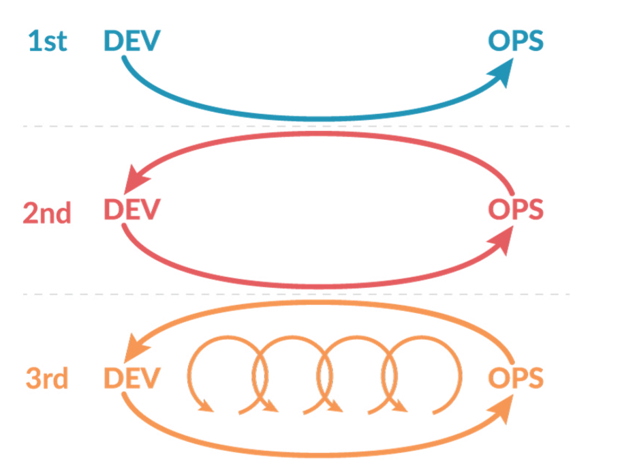
\includegraphics[width=0.6\textwidth]{Graphics/three_ways}
\caption{The Three Ways \cite{curra:2020}}
\end{figure}

Der erste Weg beschäftigt sich zu Beginn damit, den \textit{Flow} zwischen Prozessen zu verbessern. Gemeint ist damit die \glqq reibungslose, direkte Zusammenarbeit\grqq \cite{nine:2018}. Wichtig ist hierbei bereits Transparenz zu etablieren. Es muss eine Stelle geben, beispielsweise ein Sprint-Planning-Board oder ähnliches, über das alle Beteiligten auf einen Blick Einsicht erhalten über alle laufenden Prozesse, und vor allem auch wie dort der Fortschritt aussieht oder welche Probleme und Hindernisse es aktuell gibt. Die Zusammenarbeit soll verbessert werden und eine schnellere Auslieferung eine Produktiteration an den Kunden gewährleistet werden.

Der zweite Weg baut nun Feedback ein, das in jeden Prozess verankert werden soll. Dadurch wird gewährleistet dass Fehler schneller identifiziert und beseitigt werden können, ohne dass sich daraus gegebenenfalls größere Probleme entwickeln. Hiermit gilt es nicht nur den Informationsfluss zu verbessern, sondern auch um die Zusammenarbeit zu stärken und ein möglichst fehlerfreies Produkt liefern zu können. Ein wichtiger Faktor in diesem Schritt ist das Denken. Denn hier muss sich aktiv in die Rollen anderer Beteiligter hineinversetzt werden, um die \glqq Wall of Confusion\grqq , beziehungsweise das schädliche \glqq über den Zaun werfen\grqq\ eines Produktes an eine weiterführende Abteilung zu verhindern. Das Bewusstsein für die Anforderungen der Prozesskette um mich herum, und auch für den Nutzer meines Produktes soll hier in den Fokus gestellt werden, um ein Gegeneinander aus der Unternehmenskultur zu löschen.

Der letzte Schritt in diesem Konzept ist das Einbauen von Experimenten, sowie folglich die Akzeptanz von Fehlern sowie Misserfolgen. Durch Experimentieren mit neuen Wegen soll die Lernfähigkeit, aber auch die Leistungsfähigkeit der Mitarbeiter gesteigert werden. Eine zentrale Rolle spielt hierbei das Etablieren einer Vertrauenskultur, die einen Mitarbeiter auch dazu ermutigt Neues auszuprobieren. Das heißt die notorische Konnotation von Fehlern muss überwunden werden. Die so erzielten Erfolge, sowie Misserfolge, helfen beim Vorankommen und Optimieren. Hierbei kann es hilfreich sein Zeit einzuplanen bei der es ausschließlich um das Betrachten des aktuellen Standes, sowie der Erfolge und Misserfolge geht, um einen Prozess nachhaltig zu verbessern. Experimentieren mit mehreren Lösungsansätzen ist erwünscht, da nur so für den eigenen individuellen Anwendungsfall echte Ergebnisse verglichen werden können. Eine enorm wichtige Umstellung in diesem Schritt ist auch das bisherige Modell der Beziehung zu einem Manager. Dieser muss weg aus seiner Rolle des Befehle erteilens, und hin zur Interaktion mit den Mitarbeitern, die ihre eigenen Ideen und Anreize entwickeln und ausprobieren sollen.

\section{IDC DevOps Studie \cite{idc:2020}}

Um einmal einen Blick dafür zu gewinnen, ob \ac{DevOps} nun tatsächlich Anwendung findet, und vorallem wie weit es verbreitet ist, wird einmal die Studie der \ac{IDC} betrachtet. 

Die Studie wurde 2020 veröffentlicht und beschreibt nach einer Befragung von Unternehmen, wie viele von diesen DevOps Prozesse verwenden. Ganze 77\% gaben an, dass sie DevOps-Prozesse nutzen. Natürlich muss man diese Zahl mit Vorsicht genießen, da sie lediglich auf der Aussage der Befragten beruht. Dennoch ist dies schon ein enormer Anstieg. 2018, das selbe Jahr in dem auch der Heise Artikel \glqq DevOps funktioniert nicht\grqq \cite{weiss:2018} veröffentlicht wurde, gaben noch 45\% Prozent der Befragten an, DevOps-Prozesse zu verwenden.

89\% der Befragten modernisieren ihre Applikationen mithilfe einer Cloud. Der Trend weg von klassischen Architekturen, hin zu cloud-nativen Konzepten wie Container, Microservices oder auch serverlose Architekturen greifen nach DevOps als methodische Grundlage für die Arbeit mit den immer stärker entkoppelten Teilprozessen.

Von den 77\% die DevOps-Prozesse nutzen, entwickeln lediglich 19\% mehr als die Hälfte ihrer Applikationen mithilfe von DevOps. Allerdings gaben auch hier wiederum knapp 60\% der Befragten an, dass sie innerhalb von 2 Jahren mehrheitlich auf DevOps setzen wollen.

Leider stellt wie in \autoref{img:hindernisse} zu sehen, der Widerstand gegen Veränderung immer noch ein großes Problem dar beim Vorankommen von DevOps. Das liegt auch grundlegend daran, dass DevOps Mehraufwand bedeutet, und mit diesem auch einen großen Wandel einläutet, den viele Unternehmen oder Managementebenen nicht bereit sind einzugehen.

\begin{figure}[h]
\centering
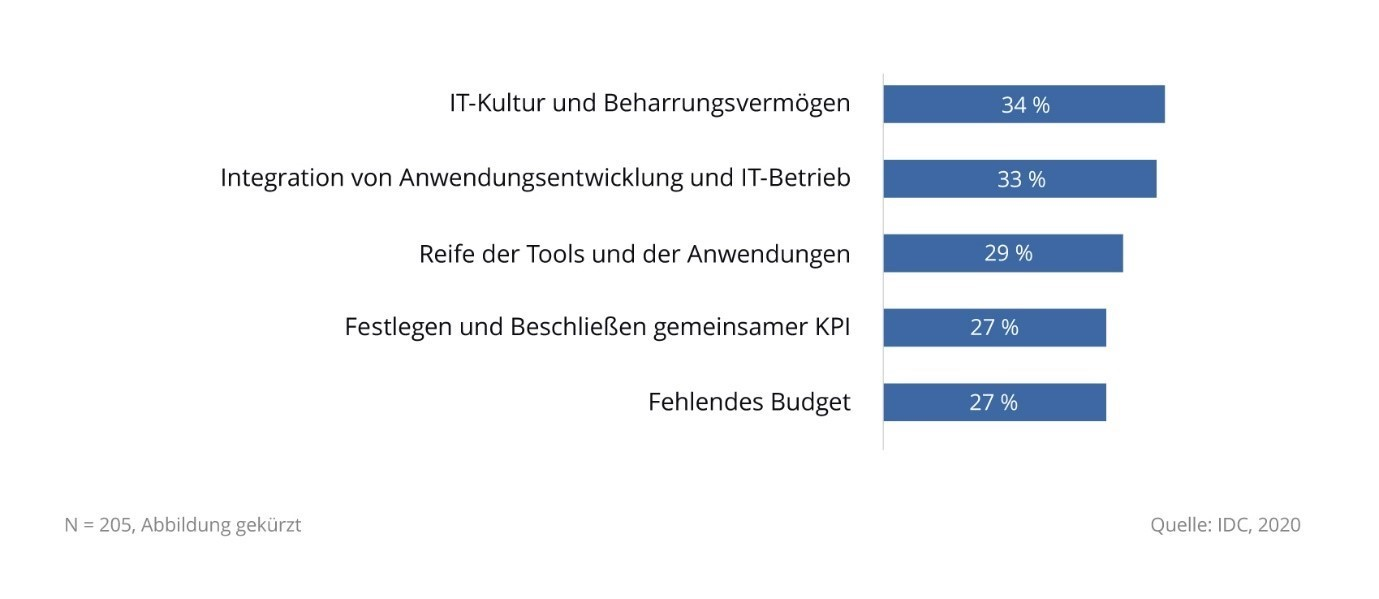
\includegraphics[width=0.9\textwidth]{Graphics/idc_hindernisse}
\caption{Hindernisse für DevOps \cite{idc:2020}}
\label{img:hindernisse}
\end{figure}

Hinzu kommt, dass der wahre Nutzen von DevOps auch auf ein gesamtes Unternehmen abgeleitet werden kann, aber zu oft als eine Spielerei für die IT abgestempelt wird. Über ein Viertel der Befragten gab an, dass das Festlegen von Kennzahlen zur Bestimmung des Nutzens über die Abteilungen hinweg sei das größte Problem bei der Einführung von DevOps gewesen. Die \ac{IDC} aber auch \citeauthor*{halstenberg:2020} \cite{halstenberg:2020} schlagen also vor, DevOps erst einmal anhand von kleinen, transparenten Projekten auszuprobieren. So kann früh ein Nutzen festgestellt werden, ohne gleich großen Aufwand oder Umstellungen zu betreiben. Von dort aus können dann langsam größere Projekte angegangen werden. So wird vermieden direkt ein zu großes Ziel in Angriff zu nehmen, an dem man ohne Erfahrung dann auch schnell scheitert und DevOps dann sofort abstempelt. Die \ac{IDC} ist sich sicher, wer jetzt Erfahrungen sammelt, und die Misserfolge und Risiken bei der Einführung von DevOps eingeht, der nutzt eine riesige Chance und wird in Zukunft zu den agilen Unternehmen gehören \glqq die als erstes, am schnellsten und am intelligentesten auf Änderungen reagieren werden.\grqq \cite{idc:2020}
